\chapter{非平行语料的语音转换}

\section{引言}
上文已经介绍了语音转换的典型框架及其各部分的主要技术,其中对于频谱转换方法主要介绍了平行语料下的
语音转换方法如混合高斯模型法,码本映射法,频率弯折法和神经网络法。随着语音转换技术的不断发展,
目前在平行语料下已经可以得到比较自然的转换声音了,然而在语音转换的实际应用中,平行语料的获取
往往需要搜集大量网络数据并从中匹配原始和目标的平行数据对,甚至原始或目标说话人亲自录制平行语料,
同时还需要尽可能保证训练数据与实际测试数据的环境条件相同,
这些都大大增加了语音转换模型的构造成本。相比平行语料而言,非平行语料的获取成本会低很多,对于知名度较高
的说话人,往往可以搜集到大量非平行语料数据。因此,基于非平行语料的语音转换方法更符合语音转换任务的实际需求。
为了与实际应用相结合,研究人员在近两年提出了许多能够实现非平行语料的频谱转换方法。如今,非平行语料正在成为语音转换的
研究热点和难点。

本章将主要介绍非平行语音转换及当前常见的频谱转换方法,包括基于音素后验概率图的方法,对抗训练法以及变分自编码器法。
之后将重点介绍基于CycleGAN的语音转换方法,该方法是非平行语料的语音转换方法中使用较为广泛的一种,也与本文的研究工作
密切相关。

\section{非平行语料语音转换概述}
非平行语料的语音转换(Non-parallel Voice Conversion)是指在原始和目标说话人的训练数据不包含相同的文本内容的条件下,
构造语音转换模型。在语音分析合成方法和韵律转换方法上,两者没有本质区别。然而不同于平行语料的语音转换,非平行语料的语音转换属于无监督任务,对于原始说话人的每一句话,并不存在对应
的标签,因此模型需要通过额外模型的帮助或特殊的训练方法来实现从两个说话人的特征中学习说话人信息并转换。非平行语料语音转换通常不需要特征对齐的步骤,两者的主要差别在频谱转换方法中。
早期的非平行语料语音转换方法以自适应的方法为主\cite{mouchtaris2004non,lee2006map}。如最早于2004年提出\cite{mouchtaris2004non},
作者在基于GMM的语音转换方法上,先使用已有的说话人平行语料预训练一个转换模型,
然后再将非平行语料的原始和目标说话人分别对转换模型做说话人自适应,从而实现非平行语料的语音转换。
另一种可行的办法是使用语音合成中的单元选择(Unit Selection)技术\cite{sundermann2006text},
从目标特征中选择与原始特征最匹配的特征帧,来实现无监督的语音转换。为了保证声学特征的连续性,当前帧的值由匹配目标帧和上一帧
加权决定。

随着近两年非平行语料的语音转换关注度增加,研究人员基于神经网络技术提出了一些更为有效的解决方案。如音素后验概率图法,
对抗训练法和变分自编码器法。其中,基于循环一致性生成对抗网络(CycleGAN)的语音转换方法在不需要任何额外数据和模型
的前提下,实现了与平行语料转换方法接近的转换性能。下文将详细介绍这些方法。

\section{常见特征转换方法}
\subsection{音素后验概率图法}
音素后验概率图法(Phonetic PosteriorGrams, PPGs)最早于2016年提出,是一种可以实现任意原始说话人到特定目标说话人(Any-to-One)的语音转换方法\cite{sun2016phonetic}。
该方法的核心思想是使用一个说话人无关特征作为中间特征,来作为原始和目标声学特征之间的媒介。通过说话人无关特征的提取器可以从任意原始说话人的语音中提取中间特征,然后只需要训练
一个从说话人无关特征到目标说话人声学特征之间的映射模型便可以实现语音转换。最直观的说话人无关特征即是文本特征,因此文章中使用每一帧对应的音素后验概率图作为中间特征,
并用语音识别系统(Automatic Speech Recognition, ASR)作为该特征的提取器。

\begin{figure}[!htp]
    \centering
    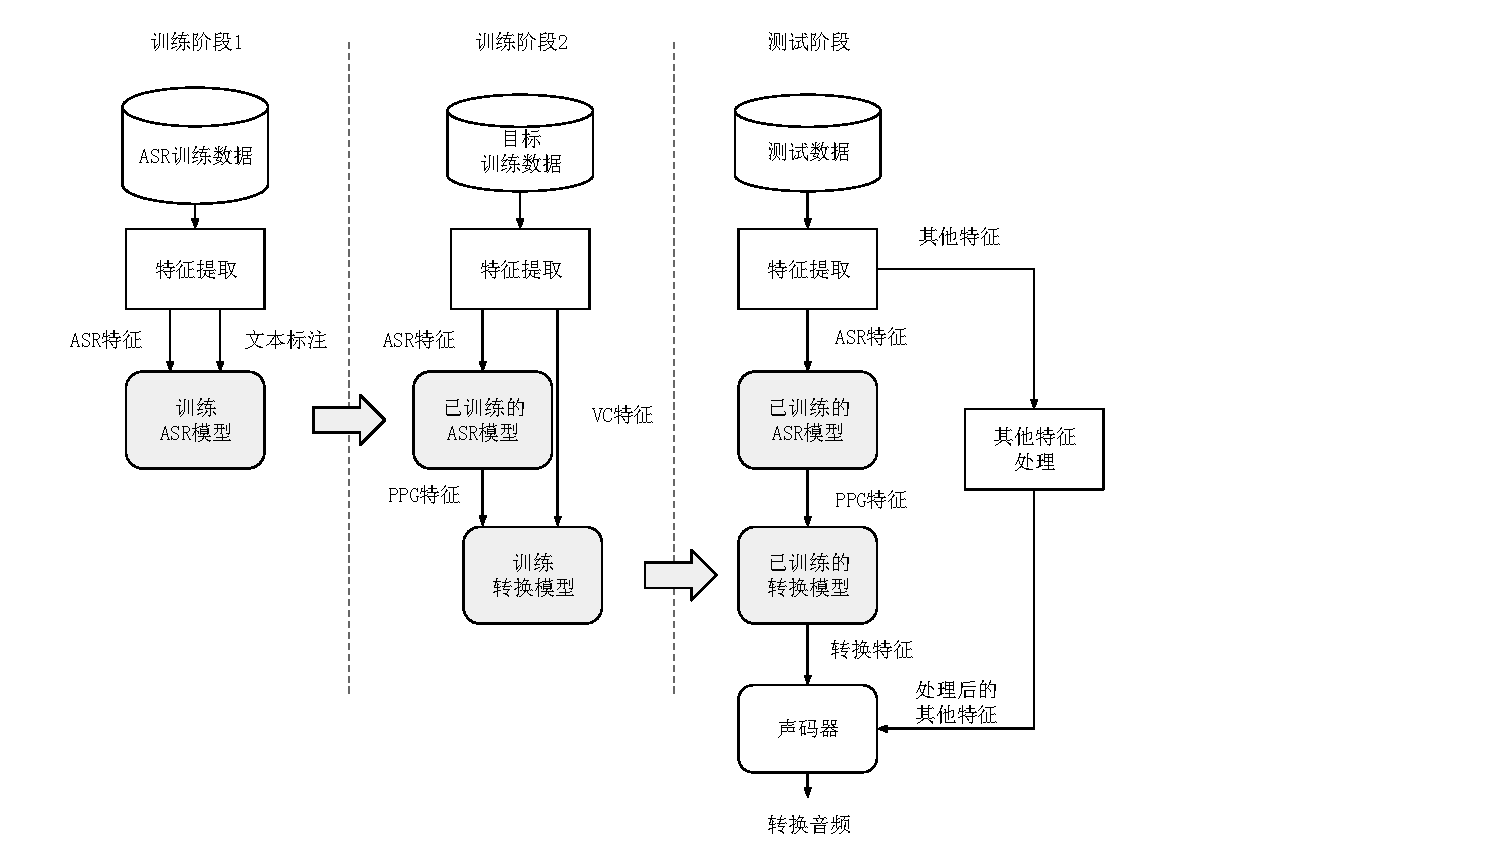
\includegraphics[width=13cm,trim=10 0 160 0,clip]{figure/3_ppg.pdf}
    \bicaption[音素后验概率图语音转换方法示意图]
    {音素后验概率图语音转换方法示意图}
    {Schematic diagram of the Phonetic PosteriorGrams Voice Conversion method}
    \label{fig:ppg}
\end{figure}

如图~\ref{fig:ppg}所示,基于PPG的语音转换方法可以分为三个模块:训练模块一,训练模块二和转换模块。在训练模块一中,使用标准的
语音识别数据集训练说话人无关的语音识别系统,这里需要用到语音识别中的声学特征如梅尔频率倒谱系数(MFCC)或滤波器组(Filter Bank, FBank)。
语音识别模型的训练可以依靠Kaldi开源工具\cite{povey2011kaldi}完成。在训练模块二中,首先对目标说话人的训练数据分别提取
ASR声学特征和VC声学特征,两个特征帧数需要保持一致。之后语音识别模型从ASR特征中预测每一帧对应的PPG特征,并用基于神经网络的
转换模型学习从PPG到VC声学特征的映射关系。在测试阶段,从原始音频中提取ASR特征,再使用ASR模型和转换模型将其依次转换为PPG特征和VC特征,
最后结合线性变换的基频和非周期信号,用WORLD声码器合成转换语音。

当前方法在实践中存在一个主要问题,由于该方法可以实现任意原始说话人的语音转换,因此在训练阶段并没有原始说话人的训练数据,而在测试时却
需要对基频进行线性变换。可能的解决方法是直接以当前句子为单位,将该句的基频分布作为原始说话人的分布。
2018年作者使用Griffin Lim(GL)声码器来合成声音,即直接从PPG中预测包含基频信息的频谱。为此作者在此基础上提出两个改进,一是将
PPG与原始对数基频序列拼接到一起作为转换模型的输入,加入原始基频信息可以帮助模型学习到频谱中基频的隐式表达,从而转换出更为自然的基频轨迹;
二是对于频谱的较高维度,建模难度较大,因此作者将频谱分为多个有重合的子带,每个子带使用一个单独的转换模型建模。测试时每个转换模型输出对应的
子带频谱后,对这些子带频谱加海明窗后拼接在一起,得到转换频谱。

随着WaveNet的提出,基于PPG的方法在WaveNet声码器下也做出了改进。对于语音转换和语音合成来说,
模型生成的声学特征和真实特征往往有一定差距,而神经网络声码器的训练特征往往都是真实特征,
因此在测试时生成的声学特征往往会导致转换语音音质的明显下降。基于此问题,
作者提出在基本框架上去除声学特征的约束,直接PPG作为WaveNet的条件特征。即将转换模型改为条件网络,和声码器共同训练。
其中转换网络由两个包含自注意力和BLSTM的模块组成。




\subsection{对抗训练法}
对抗训练法主要是指由循环一致性生成对抗网络(Cycle-consistency Generative Adversarial Networks,CycleGAN)为代表的一系列工作。
基于CycleGAN的语音转换方法于2017年提出,该方法以对偶学习为基础,包含两个互为对偶的生成模型,两个对偶模型相互串联,可以
得到两个循环来对特征进行重建,同时加入判别器对重建的中间结果进行约束,实现无监督训练。在测试阶段,只需要四个模型中的其中一个
生成器作为转换模型,转换流程与标准的语音转换方法没有本质差别。下一节将详细介绍CycleGAN的内部结构和训练机制。

针对多说话人到多说话人(Many-to-Many)的语音转换,作者于2018年提出了基于StarGAN的语音转换方法。该方法可以实现同一个模型对
原始说话人集合和目标说话人集合中的任意说话人对进行语音转换。StarGAN由一个生成器$G$,一个判别器$D$和一个分类器$D$组成。
在训练阶段,三个模型同时训练,受三个损失函数监督,分别是对抗损失,领域分类损失和循环一致性损失。
设输入特征序列为$\mathbf{x}\in \mathbb{R}^{Q\times N}$,目标属性标签为$c$,对抗损失可以公式表示为

\begin{align}
    L^D_{adv}(D) = & -\mathbb{E}_{c\sim p(c),\mathbf{y}\sim p(\mathbf{y}|c)}\left[ log D(\mathbf{y}, c) \right] \\
                   & -\mathbb{E}_{\mathbf{x}\sim p(\mathbf{x}),c\sim p(c)}\left[ log(1-D(G(\mathbf{x},c),c)) \right] \\
    L^G_{adv}(G) = & -\mathbb{E}_{\mathbf{x}\sim p(\mathbf{x}),c\sim p(c)}\left[ log D(G(\mathbf{x},c),c) \right]
\end{align}

其中$\mathbf{y}\sim p(\mathbf{y}|c)$表示已知类$c$后的真实样本集合。
对于生成器和对抗器分别有不同的对抗损失,生成器尽可能生成足够真实的类$c$样本来欺骗判别器,另一方面判别器尽可能准确地区分真实类$c$样本和生成器
生成出来的样本,判别损失可以通过对抗训练不断优化生成器和判别器,它可以帮助生成器生成接近目标分布的特征。
领域分类损失可以表示为

\begin{align}
    L^C_{cls}(C) = & -\mathbb{E}_{c\sim p(c),\mathbf{y}\sim p(\mathbf{y}|c)}\left[ log p_C(c|\mathbf{y}) \right] \\
    L^G_{cls}(G) = & -\mathbb{E}_{\mathbf{x}\sim p(\mathbf{x}),c\sim p(c)}\left[ log p_C(c|G(\mathbf{x},c)) \right] \\
\end{align}

其中$p_C(c|\mathbf{y})$表示特征序列$\mathbf{y}$属于类$c$的概率。由公式可知,在训练阶段,分类器要尽可能准确识别真实特征所属的类别。
而生成器要尽可能生成让分类器分类正确的类$c$样本。循环一致性损失如下所示

\begin{equation}
    L_{cyc}(G) = \mathbb{E}_{c^{'}\sim p(c),\mathbf{x}\sim p(\mathbf{x}|c^{'}),c\sim p(c)}\left[ \left| \left| G(G(\mathbf{x},c),c^{'})-\mathbf{x} \right| \right|_{\rho} \right]
\end{equation}

其中$c$和$c^{'}$代表两个不同的类别,$\rho$是一个正整数。另外为了在转换过程中尽可能保留语义信息,会额外添加一个身份损失,表示如下

\begin{equation}
    L_{id}(G) = \mathbb{E}_{c^{'}\sim p(c),\mathbf{x}\sim p(\mathbf{x}|c^{'})}\left[\left| \left| G(\mathbf{x},c^{'})-\mathbf{x} \right| \right|_{\rho} \right]
\end{equation}

身份损失通常在训练的初始阶段添加,可以有效缩小模型参数空间,加速收敛。为了进一步提升StarGAN-VC的性能,
作者于2019年提出了StarGAN-VC2\cite{kaneko2019stargan}。文中首先对模型的输入添加了额外的原始领域标签,
使得模型的输入是原始-目标标签对,而不是只有目标标签;其次作者使用了基于调制的加入条件特征方法,传统的加入条件的方法
通常是将条件向量与网络层的输入进行拼接或相加,但是这样做的不足是只改变了当前特征的一个维度,模型需要靠这一个维度来
输出截然不同的结果,因此作者将条件向量变为该类别所对应的均值,方差。网络的条件是有限的,对于每一组条件,都对应两个
值,分别代表均值和方差。添加条件时,先对当前特征进行归一化,然后再通过条件变量转变为另一分布,表示如下

\begin{equation}
    CIN(\mathbf{f};c^{'})=\gamma_{c^{'}}(\frac{\mathbf{f}-\mu(\mathbf{f})}{\sigma(\mathbf{f})})+\beta_{c^{'}}
\end{equation}

其中$\mathbf{f}$表示特征矩阵,$\mu$和$\sigma$分别代表特征矩阵的均值和方差,$\beta$和$\gamma$分别表示条件对应的
均值和方差。

\subsection{变分自编码器法}

\begin{figure}[!htp]
    \centering
    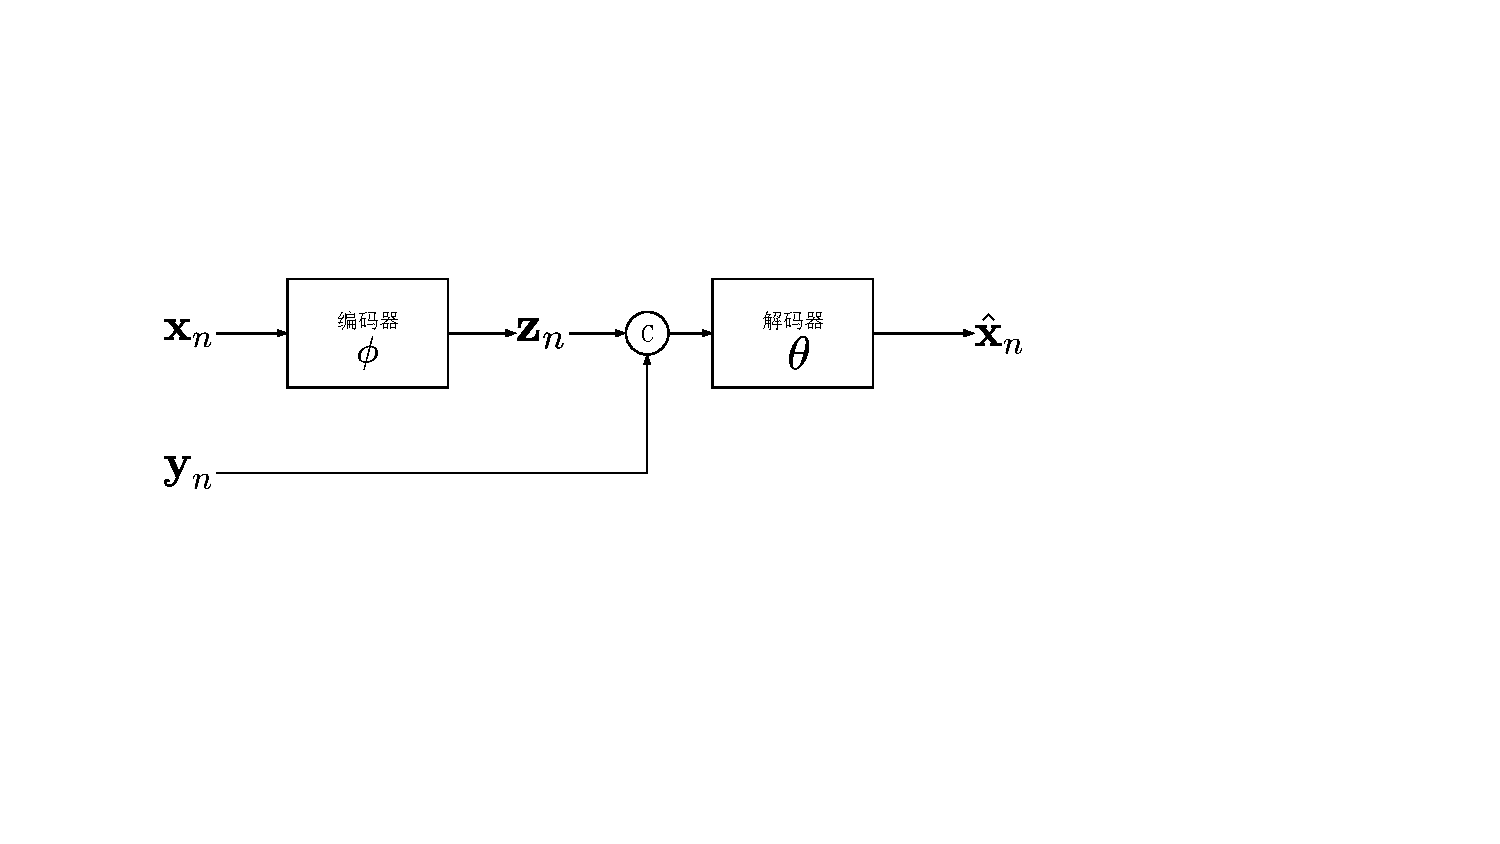
\includegraphics[width=13cm,trim=30 170 170 130,clip]{figure/3_vae.pdf}
    \bicaption[变分自编码器语音转换方法示意图]
    {变分自编码器语音转换方法示意图}
    {Schematic diagram of the VAE Voice Conversion method}
    \label{fig:vae}
\end{figure}

基于变分自编码器(Variational AutoEncoder, VAE)的语音转换方法于2016年被提出。VAE同生成对抗模型类似,也是生成模型的一种。
如图~\ref{fig:vae}所示,VAE可以分为编码器$\phi$和解码器$\theta$两个模型,其中编码器将输入的声学特征$\mathbf{x}_n$转换为说话人无关的隐变量$\mathbf{z}_n$:

\begin{equation}
    \mathbf{z}_n = f_{\phi}(\mathbf{x}_n)
\end{equation}

此时隐变量只包含说话人无关的信息,例如音素,韵律等。之后,用解码器将隐变量恢复为最初的输入$\mathbf{x}_n$,为此,需要额外添加说话人信息变量$\mathbf{y}_n$。
解码器以隐变量和说话人信息拼接之后的结果作为输入,即

\begin{equation}
    \hat{\mathbf{x}}_n = f_{\theta}(\mathbf{z}_n,\mathbf{y}_n)
\end{equation}

基于VAE的语音转换方法基于两个假设:一是说话人信息和说话人无关信息可以从一帧声学特征向量中解耦出来;二是解码器可以通过混合这两个信息来合成一个声学特征向量。
模型的最终目标函数可以表示为

\begin{equation}
    \hat{L}(\theta,\phi,x_n)=-D_{KL}(q_{\phi}(\hat{z}_n|x_n)||p(z_n))+logp_{\theta}(x_n|\hat{z}_n,y_n)
\end{equation}

在转换过程中,编码器首先将输入帧转变为隐向量,然后解码器输入隐向量和目标说话人向量来输出转换特征帧。


\section{基于CycleGAN的语音转换方法}
本文所做的语音转换工作主要基于CycleGAN的语音转换方法,本节将先简要介绍该方法涉及到的基本概念如对偶学习,生成对抗网络等,
之后对CycleGAN的原理及其在语音转换上的优化进行详细说明。

\begin{figure}[!htp]
    \centering
    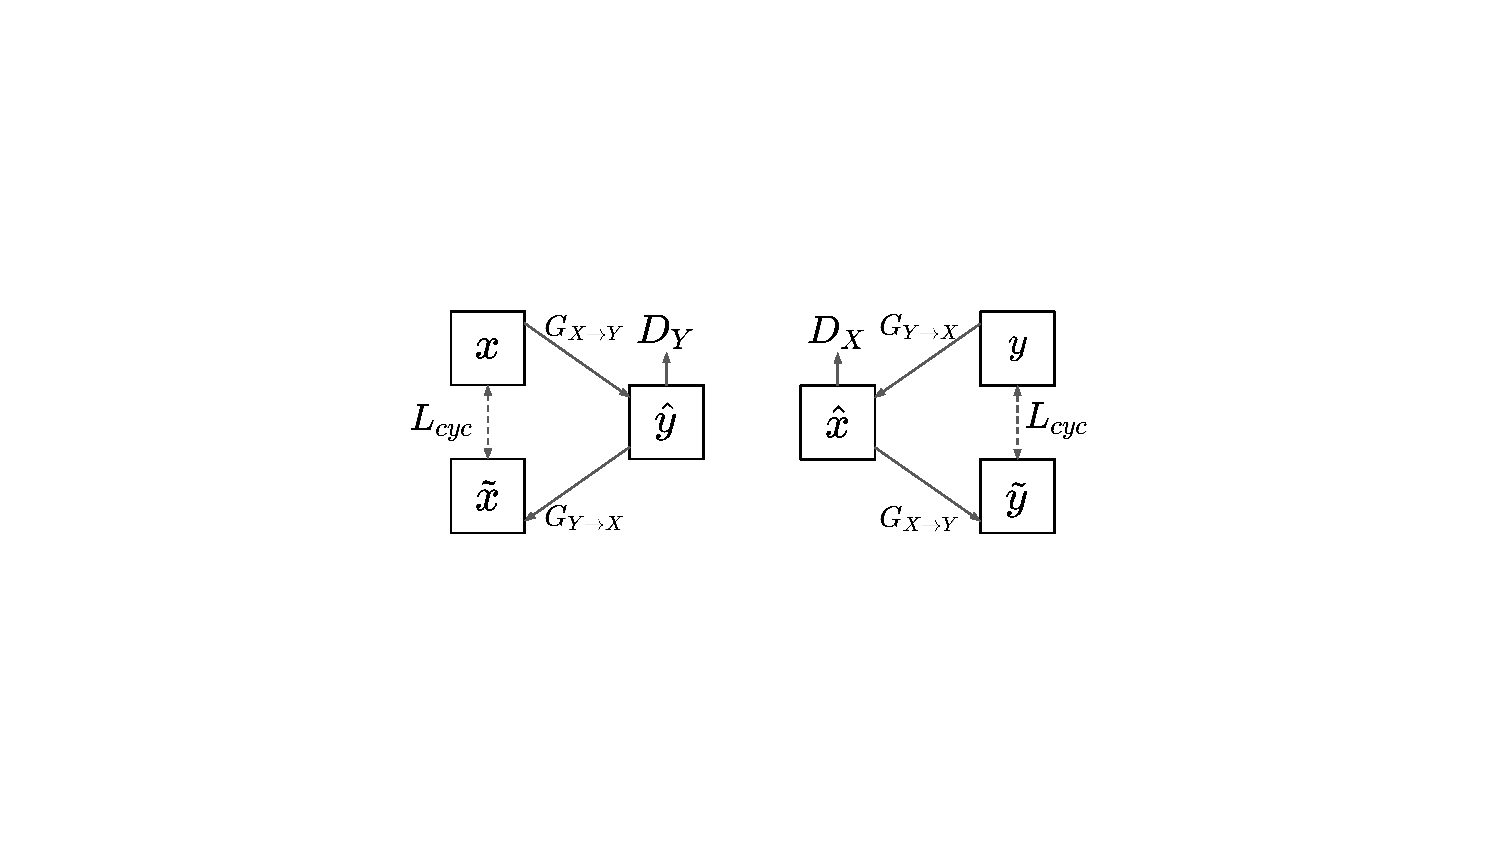
\includegraphics[width=13cm,trim=100 140 100 140,clip]{figure/3_cyclegan.pdf}
    \bicaption[标准CycleGAN示意图]
    {标准CycleGAN示意图}
    {Schematic diagram of the standard CycleGAN}
    \label{fig:cyclegan}
\end{figure}

\subsection{对偶学习概述}
对偶学习(Dual Learning)的概念最早于2016年提出\cite{he2016dual}。以神经网络为代表的深度学习技术
近两年在许多领域内都取得了巨大的成功,其中一个重要的因素就是大数据,尤其是大规模的经过标注的数据。例如
在语音合成中,神经网络通常需要上万句带有标注的音频样本来学习文本到声学特征之间的关系,这些数据需要
大量人工对其进行标注,校对等工作,极大增加了一个模型的构建成本。这个问题在机器翻译领域尤为突出,在机器
翻译中,会用到上千万的双语句对进行训练,这对数据的收集和标注都提出了很大的挑战。深度学习技术的广泛性
与其对大规模标注数据的依赖性有很大的关系。为了解决这个问题,研究人员提出了一种新的学习范式,即对偶学习。

可以发现,很多深度学习的任务都可以衍生出一个对偶任务,如机器翻译的中译英和英译中,语音转换的原始说话人转目标说话人和
目标说话人转原始说话人,甚至语音识别和语音合成。这些互为对偶的深度学习任务可以形成一个闭环,使从没有标注的数据中学习
模型成为可能。对偶学习最重要的一点是,对于一个主任务,其对偶任务可以给其反馈,反过来主任务也可以给对偶任务以反馈,从而
实现两个任务相互反馈,相互学习。

实际上对偶学习与强化学习的学习过程较为相似。在强化学习中,并没有标注样本来告诉模型在某个状态执行某个动作是正确的,模型
只有通过使用策略在某个状态下执行不同的动作,观测该动作带来的回报,从而改善策略。在对偶学习中,两个对偶任务就是策略,
模型输入就是状态,两次模型的输出就是动作,而重建误差就是动作带来的回报。

以中英机器翻译为例,已有预训练或未训练的英译中模型$f$和中译英模型$g$,给定一个英文句子$x$,首先用英译中模型$f$将该句翻译成中文$y^{'}$,
然后将该中文句子$y^{'}$发送给中译英模型$g$。中译英模型$g$并不知道正确的翻译是什么,但可以知道这个中文句子语法是否正确,
是否符合中文语言模型,这些信息都可以帮助中译英模型$g$判断英译中模型$f$是否做的好。然后中译英模型$g$翻译成英文句子$x^{'}$,
通过比较$x$和$x^{'}$是否相似,就可以判断两个模型$f$和$g$做的是不是足够好,尽管输入$x$是一个没有标注的句子。同理,也可以输入
中文句子,使其分别通过中译英模型$g$和英译中模型$f$,来实现重建。因此,通过
这样的一个对偶游戏的过程,就能够从没有标注的数据上获得反馈,从而提高模型性能。

对偶学习同样可以应用在语音转换中,对于语音转换而言,原始说话人和目标说话人可以互相调换,来得到对应的对偶任务。
为了训练从说话人$A$到说话人$B$的语音转换模型$G$,需要同时学习转换模型$G_{A\rightarrow B}$和$G_{B\rightarrow A}$。
分别输入两个说话人的原始特征,通过两个模型对原始特征进行重构,将重构误差作为回报帮助两个模型训练。但是仅有重构误差对于语音转换
的对偶学习来说还是不够的,因为两个模型很容易都训练成将输入原样输出来使重构误差最小,为了解决这个问题,需要在每次循环中对第一个模型
的输出加入约束,强制其输出符合目标说话人的特征分布。

\subsection{生成对抗网络简介}
生成对抗网络(Generative Adversarial Networks, GAN)由Ian Goodfellow等人于2014年提出\cite{goodfellow2014generative}。
迄今为止GAN已经在许多生成式任务中实现了非常好的效果,如图像生成,自然语言生成和音乐声称等。该模型从一个游戏理论中获得启发:两个模型,
一个生成器(Generator),一个判别器(Discriminator),在互相竞争的过程中彼此越来越强大。然而,GAN的训练是较为困难的,研究人员在训练过程中经常遇到不稳定和模型不收敛的问题。

GAN包含两个模型:判别器$D$对输入样本进行判断,并输出该样本属于真实数据集的概率,判别器像一个裁判,其优化目标是对真实
样本尽可能高的概率值,同时对合成样本较低的概率值。生成器$G$输入噪声变量$z$,输出合成样本,生成去的训练目标是尽可能生成接近
真实数据分布的合成样本,以至于可以欺骗判别器,使其给出较高的概率值。在训练过程中,两个模型在这个零和游戏中互相对抗,并不断提升彼此的能力。

一方面,判别器$D$确保在真实数据上足够准确,通过最大化$\mathbb{E}_{x\sim p_r(x)}\left[log D(x)\right]$,同时,输入一个假的样本
$G(z)$,$z\sim p_z(z)$,判别器期望输出其概率$D(G(z))$尽可能接近$0$通过最大化$\mathbb{E}_{z\sim p_z(z)}\left[log(1-D(G(z)))\right]$。
在另一方面,生成器希望提升判别器对其生成的样本的概率值通过最小化$\mathbb{E}_{z\sim p_z(z)}\left[log(1-D(G(z)))\right]$。将两个目标函数
合并,可以得到需要优化的损失函数

\begin{equation}
    \min_G \max_D L(D,G)=\mathbb{E}_{x\sim p_r(x)}\left[log D(x)\right] + \mathbb{E}_{z\sim p_z(z)}\left[log(1-D(G(z)))\right]
\end{equation}

其中等号右边的第一项对生成器$G$训练时没有影响。通过对损失函数在所有x上求导,可以得到对于判别器而言,其使损失函数最低的最优概率值为0.5,整个
损失函数的全局最优值为$-2log2$。GAN的发展至今已经演变出很多种类,包括加入条件的条件GAN,使用最小二乘法的LSGAN,以及引入对偶学习的CycleGAN,StarGAN等。

\subsection{CycleGAN网络的训练}
CycleGAN网络包含四个模型,两个生成器($G_{X\rightarrow Y}$,$G_{Y\rightarrow X}$)和两个判别器($D_X$,$D_Y$),$X$和$Y$分别代表原始域和目标域。
四个模型通过两个个损失函数来实现无监督的训练:对抗损失(Adversarial Loss)和重构损失(Reconstruct Loss)。
其中对抗损失用来衡量转换的目标特征和真实的目标特征之间的区分程度。判别器通过最大化对抗损失来尽可能区分转换特征和真实特征,
同时生成器通过最小化对抗损失来尽可能生成接近真实的转换特征,从而欺骗判别器。其训练方式与生成对抗网络类似,
生成器和判别器交替训练更新,训练生成器时判别器只回传梯度,不更新梯度。对抗损失表示如下

\begin{align}
    L_{adv}(G_{X\rightarrow Y},D_Y) & =\mathbb{E}_{y\sim P_{Data}(y)}\left[log D_Y(y)\right] \\
    & + \mathbb{E}_{x\sim P_{Data}(x)}\left[log(1-D_Y(G_{X\rightarrow Y}(x)))\right] \\
    L_{adv}(G_{Y\rightarrow X},D_X) & =\mathbb{E}_{x\sim P_{Data}(x)}\left[log D_X(x)\right] \\
    & + \mathbb{E}_{y\sim P_{Data}(y)}\left[log(1-D_X(G_{Y\rightarrow X}(y)))\right] 
\end{align}


对于重构损失,域$X$中的每一个样本$x$都可以通过主任务和对偶任务(或交换)的级联重新恢复为$x$,因此重构损失可以表示为

\begin{align}
    L_{cyc}(G_{X\rightarrow Y},G_{Y\rightarrow X}) & = \mathbb{E}_{x\sim P_{Data}(x)}\left[\left| \left| G_{Y\rightarrow X}(G_{X\rightarrow Y}(x))\right| \right|_1 \right] \\
    & + \mathbb{E}_{y\sim P_{Data}(y)}\left[\left| \left| G_{X\rightarrow Y}(G_{Y\rightarrow X}(y))\right| \right|_1 \right]
\end{align}

如图~\ref{fig:cyclegan}所示,输入依次经过两个级联的生成器后,得到的输出和输入计算重构损失,之后梯度沿着两个生成器反向传播,
并对两个生成器同时更新参数。对两个损失函数加入权重后,最终的损失函数为

\begin{align}
    L_{full}& =L_{adv}(G_{X\rightarrow Y},D_Y)+L_{adv}(G_{Y\rightarrow X},D_X)\\
    & +\lambda_{cyc}L_{cyc}(G_{X\rightarrow Y},G_{Y\rightarrow X})
\end{align}

\subsection{门控卷积网络和身份损失}
为了将CycleGAN应用到语音转换中,作者提出了在网络中使用门控卷积网络(Gated CNN)以及一个额外的身份损失函数(Identity Loss)。
语音中的一个主要特性就是语音中含有序列和层级的结构关系,例如发声和不发声(voiced/unvoiced),音素和词素(phonemes/morphemes)。
一个对该特性建模的有效方法是使用RNN,但是RNN在训练和计算速度上都不如CNN。因此作者提出在CycleGAN中使用门控卷积网络。门控卷积网络
既可以在序列数据上并行计算,同时也在语言和语音建模上较为成功。在门控卷积网络中,选用门控线性单元(Gated Linear Unit, GLU)作为激励函数。
GLU计算过程公式表示为

\begin{equation}
    \mathbf{H}_{l+1}=(\mathbf{H}_l \ast \mathbf{W}_l + b_l)\otimes \sigma (\mathbf{H}_l \ast \mathbf{V}_l + c_l)
\end{equation}

其中$\mathbf{W}$,$\mathbf{V}$,$b$和$c$是模型参数,$\mathbf{H}_l$是$l$层的输出,$\otimes$是逐元素乘法。门控机制可以允许信息被
选择性地传播到下一层。

身份损失通常只用来在训练的开始阶段使用,其作用为在训练开始时尽可能缩小生成器的参数空间。
该损失函数的提出考虑到对于语音转换任务而言,只需考虑转换说话人信息,而语音中的主要信息(如文本)是不改变的。
因此在训练开始时首先尽可能保证生成器保留语音中的所有信息,之后再对其中的说话人信息进行着重调整,
身份损失能够有效加速模型收敛和保留语义。为了保证生成器的输出始终在目标说话人的特征分布内,
身份损失选择输入目标特征而非原始特征。公式如下

\begin{align}
    L_{id}(G_{X\rightarrow Y},G_{Y\rightarrow X}) & = \mathbb{E}_{y\sim P_{Data}(y)}\left[\left| \left| G_{X\rightarrow Y}(y)-y\right| \right|_1 \right] \\
    & + \mathbb{E}_{x\sim P_{Data}(x)}\left[\left| \left| G_{Y\rightarrow X}(x)-x\right| \right|_1 \right]
\end{align}

\section{本章小结}
本章首先介绍了非平行语音转换及其常见方法,包括音素后验概率图法,对抗训练法和变分自编码器法,并对本文中用到的基于CycleGAN的语音转换方法
进行了详细的介绍。标准的CycleGAN中计算重构损失时,级联的两个生成器同时进行前向和后向传播。
在该设置下,转换音频通常包含有较多噪音,从而会导致较低的语音自然度和说话人相似度。
下一章将会从更新过程的角度进一步分析标准CycleGAN的训练过程,并介绍所提出的半优化CycleGAN和基频辅助特征来提升模型性能。
